\chapter{Stochastic Interventional Vaccine Efficacy}\label{three}

\section{Introduction}

The core ideas of Chapter~\ref{two} can form a novel approach to studying immune
correlates of protection --- those antibody markers causally antagonistic to the
infectious process~\citep{plotkin2012nomenclature} --- in vaccine efficacy
trials of infectious diseases. Such analyses can help to better understand which
antibody markers impact vaccine efficacy and elucidate the mechanism by which
they may afford protection. In this analytic framework, vaccine efficacy may be
quantified as the effect of shifting (upwards or downwards) the immune response
distribution in vaccinees~\citep{hejazi2020efficient}, making it possible to
develop a more nuanced understanding of the mechanism by which a vaccine
provides protection.

The data collected on a single individual in a randomized vaccine efficacy trial
may be represented by the random variable $O = (X, A, S, Y)$, where $X$ are
baseline risk factors for infection (such as age or body-mass index), $A$ is the
randomized assignment to placebo or vaccine, $S$ is the immune response activity
of an antibody of interest, and $Y$ is an indicator of infection. Throughout, we
assume that $S$ is the scalar-valued activity of a particular antibody, as
quantified by an established immunological assay, that is a candidate immune
correlate of protection.

Given the central goal to
develop a parsimonious surrogate endpoint based on a single immunoassay, the
main analysis will use each of the methods to assess each of the five
quantitative readouts (not baseline-subtracted) separately as CoPs, adjusting
for the same set of baseline covariates as used in the correlates or risk
analyses described in~\citet{gilbert2021covpn}.

\section{Formulating Vaccine Efficacy Parameters}

Each involves consideration of a binary
counterfactual outcome $Y(a,s)$ (e.g., indicator of the COVID disease endpoint
by a pre-specified time) under a hypothetical intervention that both sets
randomization assignment $A=a$ and sets the Day 57 immunologic marker $S$ to
a fixed value or based upon a random draw from a analyst-specified distribution.

Specifically, we can consider the
effect on risk of a given endpoint of a controlled intervention that shifts the
distribution of an immune response by $\delta$ units, where $\delta$ is an
analyst-specified real number. Considering a counterfactual scenario in which we
are able to intervene so as to modify the immune response induced by the vaccine
(e.g., a hypothetical change in dose or other re-formulation of the vaccine), we
take this hypothetical intervention to lead to an improved (if $\delta > 0$) or
lessened immune response (if $\delta < 0$) relative to the current vaccine (at
$\delta = 0$). Using this framework, we can query the counterfactual risk of the
endpoint under this hypothetical vaccine. Using notation established above, this
quantity can be expressed as the mean of the counterfactual variable $Y(1, S(1)
+ \delta)$.

This approach is similar to the controlled effects approach described in
Section~\ref{cop_mediation_ve}, but with an important distinction. In the
controlled effects approach, one assumes that it is possible to set $S = s$ for
\textit{all} individuals in the population. For high values of $s$, this
assumption may be unrealistic if the vaccine fails to be strongly immunogenic
for some subpopulations. On the other hand, with the interventional approach, it
is only required that individuals' immune responses be shifted relative to their
observed immune response, which may be more plausible for some vaccines. 

Under assumptions~\citep{hejazi2020efficient}, the main two of which being no
unmeasured confounding and positivity (forms of both are also required for the
Controlled VE CoP analyses), the counterfactual risk of interest 
$E[Y(1, S(1) + \delta)]$ is identified by
\[
  E[P(Y = 1 \mid A = 1, S = S + \delta, X = x) \mid A = 1, X] \ . 
\]
Examining this quantity across a range of $\delta$ provides insight into the
relative contribution of a given immune response marker in preventing the
endpoint of interest. 

\section{Considerations for Statistical Estimation}

\citet{hejazi2020efficient} proposed nonparametric estimators that rely on
estimates of the outcome regression (as described above) and the conditional
density of the immune response marker in vaccinated participants. Their
estimators efficiently account for two-phase sampling of immune responses and
are implemented in the \texttt{txshift} package~\citep{hejazi2020txshift-joss}
for the \texttt{R} language and environment for statistical computing~\citep{R},
available via both GitHub at \url{https://github.com/nhejazi/txshift} and the
Comprehensive \texttt{R} Archive Network at
\url{https://CRAN.R-project.org/package=txshift}.

These estimators will be applied to each of the five Day 57 antibody markers
(without baseline adjustment) controlling for the same set of baseline risk
factors as would be controlled for in other analyses previously discussed. As
with the mediation analysis approach described in
\citet{benkeser2021inference,gilbert2021covpn}, the procedure will leverage
low-dimensional risk factors alongside parametric regression strategies and
flexible conditional density estimators for endpoints with fewer than 100
observed cases (pooling over the randomization arms); however, more flexible
learning techniques will be employed for modeling the outcome process for
endpoints with a greater number of observed cases.

In particular, conditional density estimates of immune response markers will be
principally based on a nonparametric estimation strategy that reconstructs the
conditional density through estimates of the conditional hazard of the
discretized immune response marker values~\citep{hejazi2020efficient,
hejazi2020efficient, hejazi2020haldensify}; this approach is an extension
of the proposal of~\citet{diaz2011super}. A Super Learner
ensemble~\citep{vdl2007super} of variants of this nonparametric
conditional density estimator and semiparametric conditional density estimators
based on Gaussinization of residuals will be constructed using the \texttt{sl3}
\texttt{R} package~\citep{coyle2020sl3}. In settings with limited numbers of
case endpoints, the outcome process will be modeled as a Super Learner ensemble
of a library of parametric regression techniques~\citep[as recommend
by][]{gruber2010application}, while the library will be augmented with flexible
regression techniques --- including, for example, lasso and ridge
regression~\citep{tibshirani1996regression,tikhonov1977solutions,hoerl1970ridge},
elastic net regression~\citep{zou2003regression,friedman2009glmnet}, random
forests~\citep{breiman2001random, wright2017ranger}, extreme gradient boosting
machines~\citep{chen2016xgboost}, multivariate adaptive polynomial and regression
splines~\citep{friedman1991multivariate, stone1994use,
kooperberg1997polychotomous}, and the highly adaptive
lasso~\citep{vdl2017generally,benkeser2016highly,hejazi2020hal9001-joss} --- as
the number of endpoint cases grows. These algorithm libraries will be
coordinated to match those used in other CoP analyses.

Additionally, we recall that $P(Y(0)=1) = P(Y=1 \mid A=0)$ (in view of vaccine
versus placebo randomization, as stated previously in
Section~\ref{cop_controlled_ve}) and may be estimated in the same way as for the
analysis of controlled vaccine efficacy, thus yielding an estimate of
stochastic interventional VE defined by $$ SVE(\delta) = 1 - \frac{E[P(Y
= 1 \mid A = 1, S = S + \delta, X = x) \mid A = 1, X]}{P(Y(0)=1)}.$$

Output of the analyses will be presented as point and 95\% confidence interval
estimates of $E[Y(1, S(1) + \delta)]$ and of $SVE(s)$ over the values of $s$ for
each of the Day 57 antibody markers, for each of a range of $\delta$ spanning -2
to 2 on the standard unit scale for each antibody marker.

Lastly, just as for the controlled VE CoP analyses, these analyses will only be
performed if diagnostics support plausibility of the positivity assumption.
Importantly, however, the positivity assumption for the stochastic
interventional effects differs from that usually required. That is, where the
positivity assumption for effects defined by static interventions requires
a positive probability of treatment assignment across all strata defined by
baseline factors (i.e., that a discretized immune response value be possible
regardless of baseline factors), the positivity assumption of these effects is
$$s_i \in \mathcal{S} \implies s_i + \delta
    \in \mathcal{S} \mid A = 1, X = x$$
\noindent for all $x \in \mathcal{X}$ and
    $i = 1, \ldots n$.
In particular, this positivity assumption does not require that the
post-intervention exposure density, $q_{0,S}(S - \delta \mid A = 1, X)$,  place
mass across all strata defined by $X$. Instead, it requires that the
post-intervention exposure mechanism be bounded, i.e.,
$$P
\{q_{0,S}(S - \delta \mid A = 1, X) / q_{0,S}(S \mid A = 1, X) > 0 \} = 1,$$
\noindent which may be readily satisfied by a suitable choice of $\delta$.

More importantly, the static intervention approach may require consideration of
counterfactual variables that are scientifically unrealistic. Namely, it may be
inconceivable to imagine a world where every participant exhibits high immune
responses, given the phenotypic variability of participants' immune systems.
This too may be resolved by considering an intervention $\delta(X)$, allowing
the choice of $\delta$ to be a function of baseline covariates
$X$~\citep{hejazi2020efficient, diaz2012population, haneuse2013estimation,
diaz2018stochastic}.

We estimate the counterfactual mean of symptomatic COVID-19 infection
under posited shifts in the measured activity levels of each of 4
\emph{candidate} mechanistic correlates of protection (mCoP) biomarkers.
By shifting the \emph{standardized} biomarker activity levels by
standard unit shifts along the grid \{-1, -0.5, 0, 0.5, 1\}, we can
assess the degree to which vaccines that modulate mCoP biomarker
activity to these levels could mitigate symptomatic COVID-19 infection
in terms of counterfactual stochastic interventional risk and vaccine
efficacy (VE).

\section{Application to the COVID-19 Pandemic}

\subsection{Evaluating Spike Protein Binding Antibodies}\label{spba-day57}

\begin{figure}[H]
  \centering
  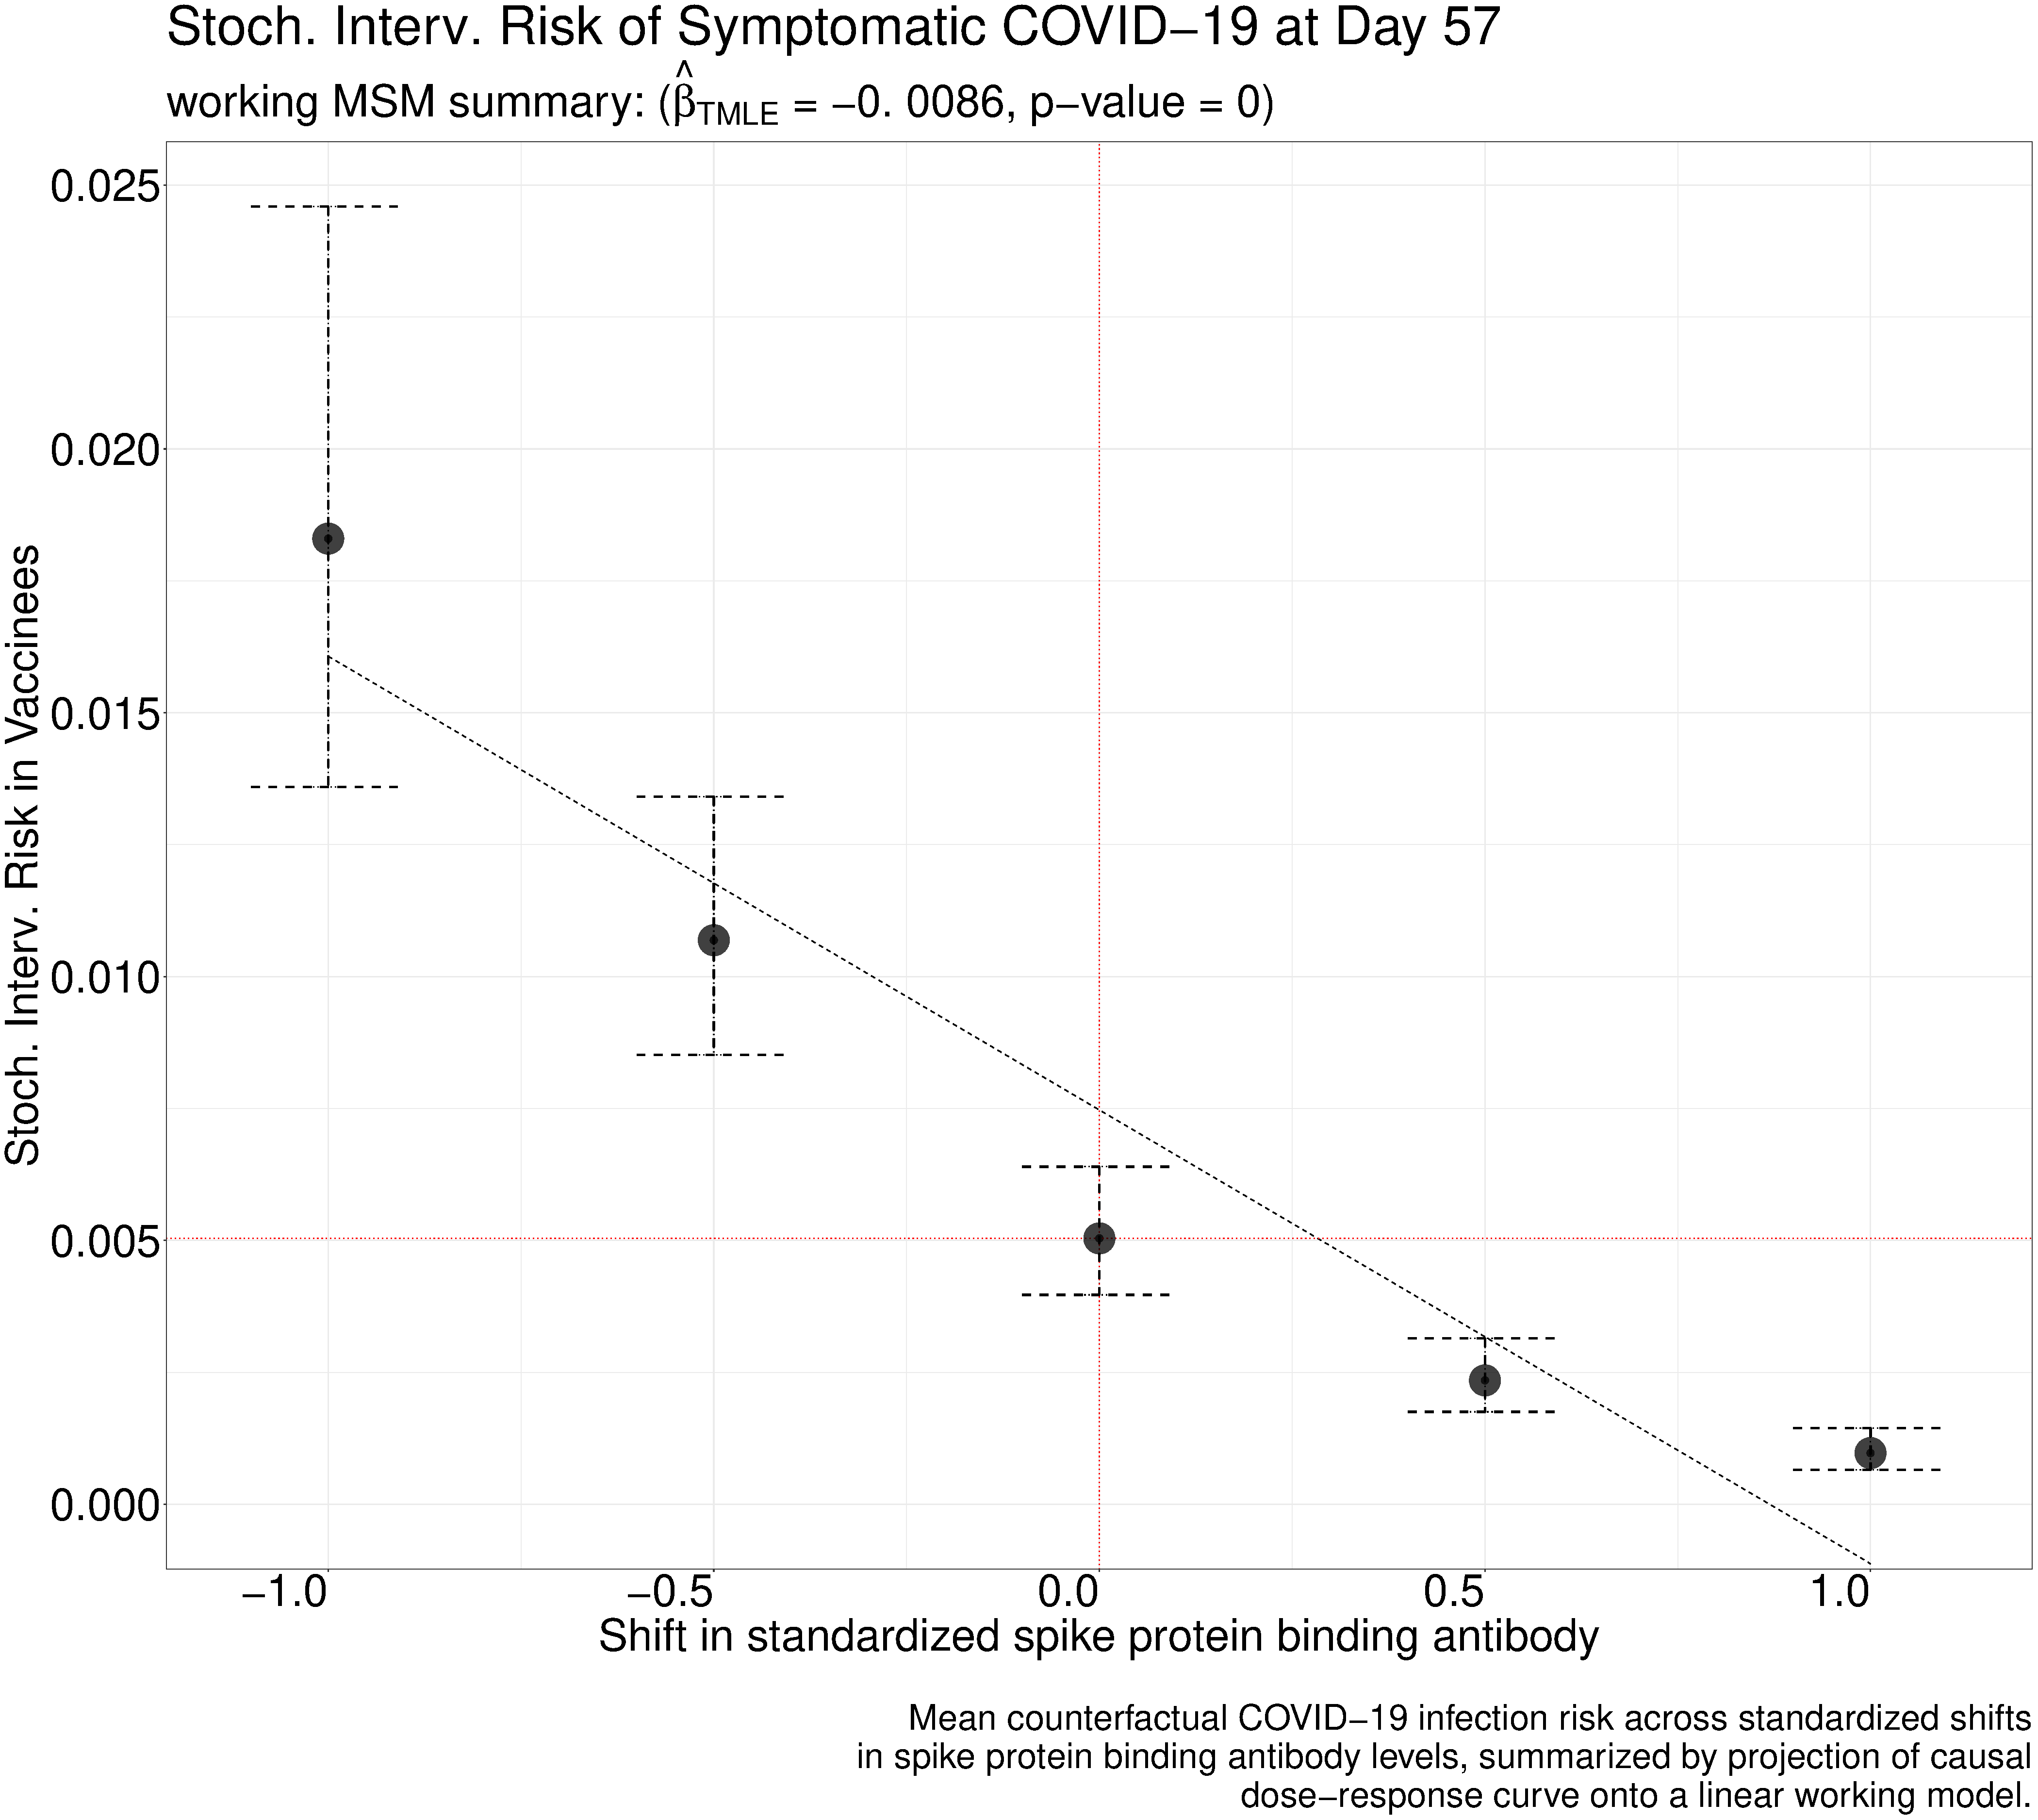
\includegraphics[width=0.95\linewidth,]{mcop_risk_Day57bindSpike}
  \caption{Stochastic interventional risk estimates, with confidence intervals,
  for spike protein binding antibody at Day 57}
  \label{fig:marker1-risk-day57}
\end{figure}

\begin{figure}[H]
  \centering
  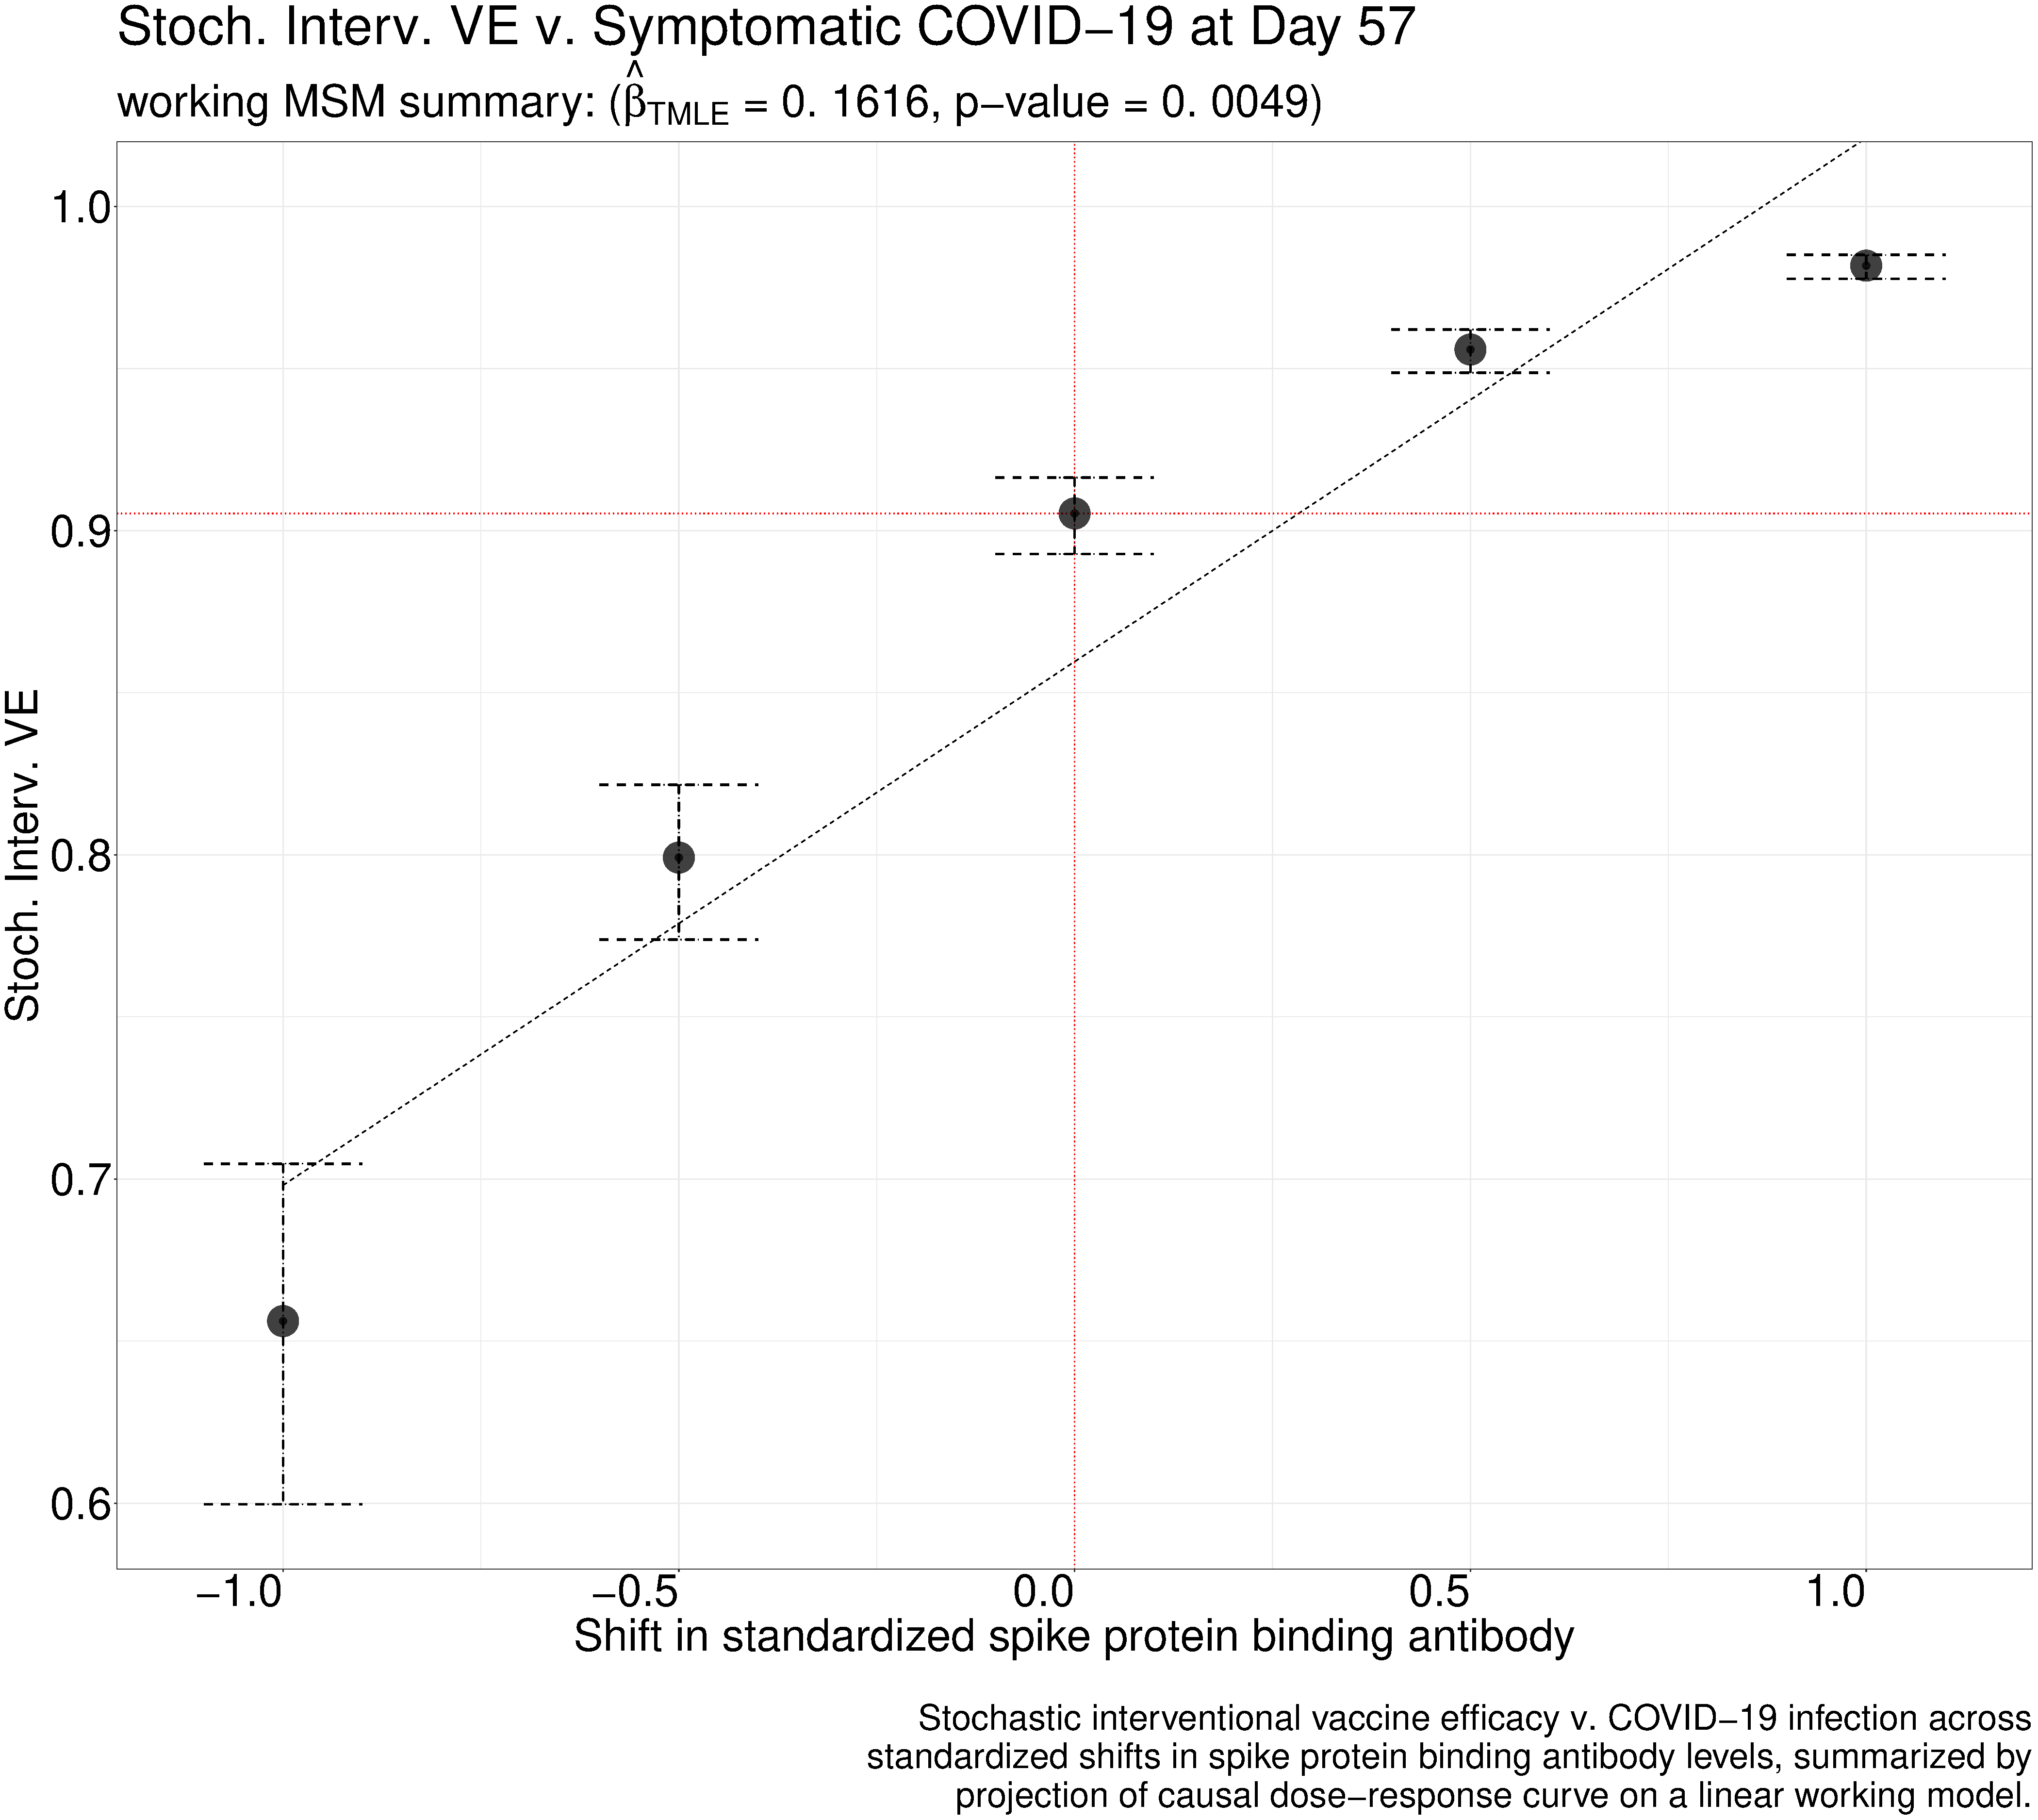
\includegraphics[width=0.95\linewidth,]{mcop_sve_Day57bindSpike}
  \caption{Stochastic interventional VE estimates, with confidence intervals,
    for spike protein binding antibody at Day 57}
  \label{fig:marker1-sve-day57}
\end{figure}

\subsection{Evaluating Pseudo-neutralizing Antibodies}\label{psna-day57}

\begin{figure}[H]
  \centering
  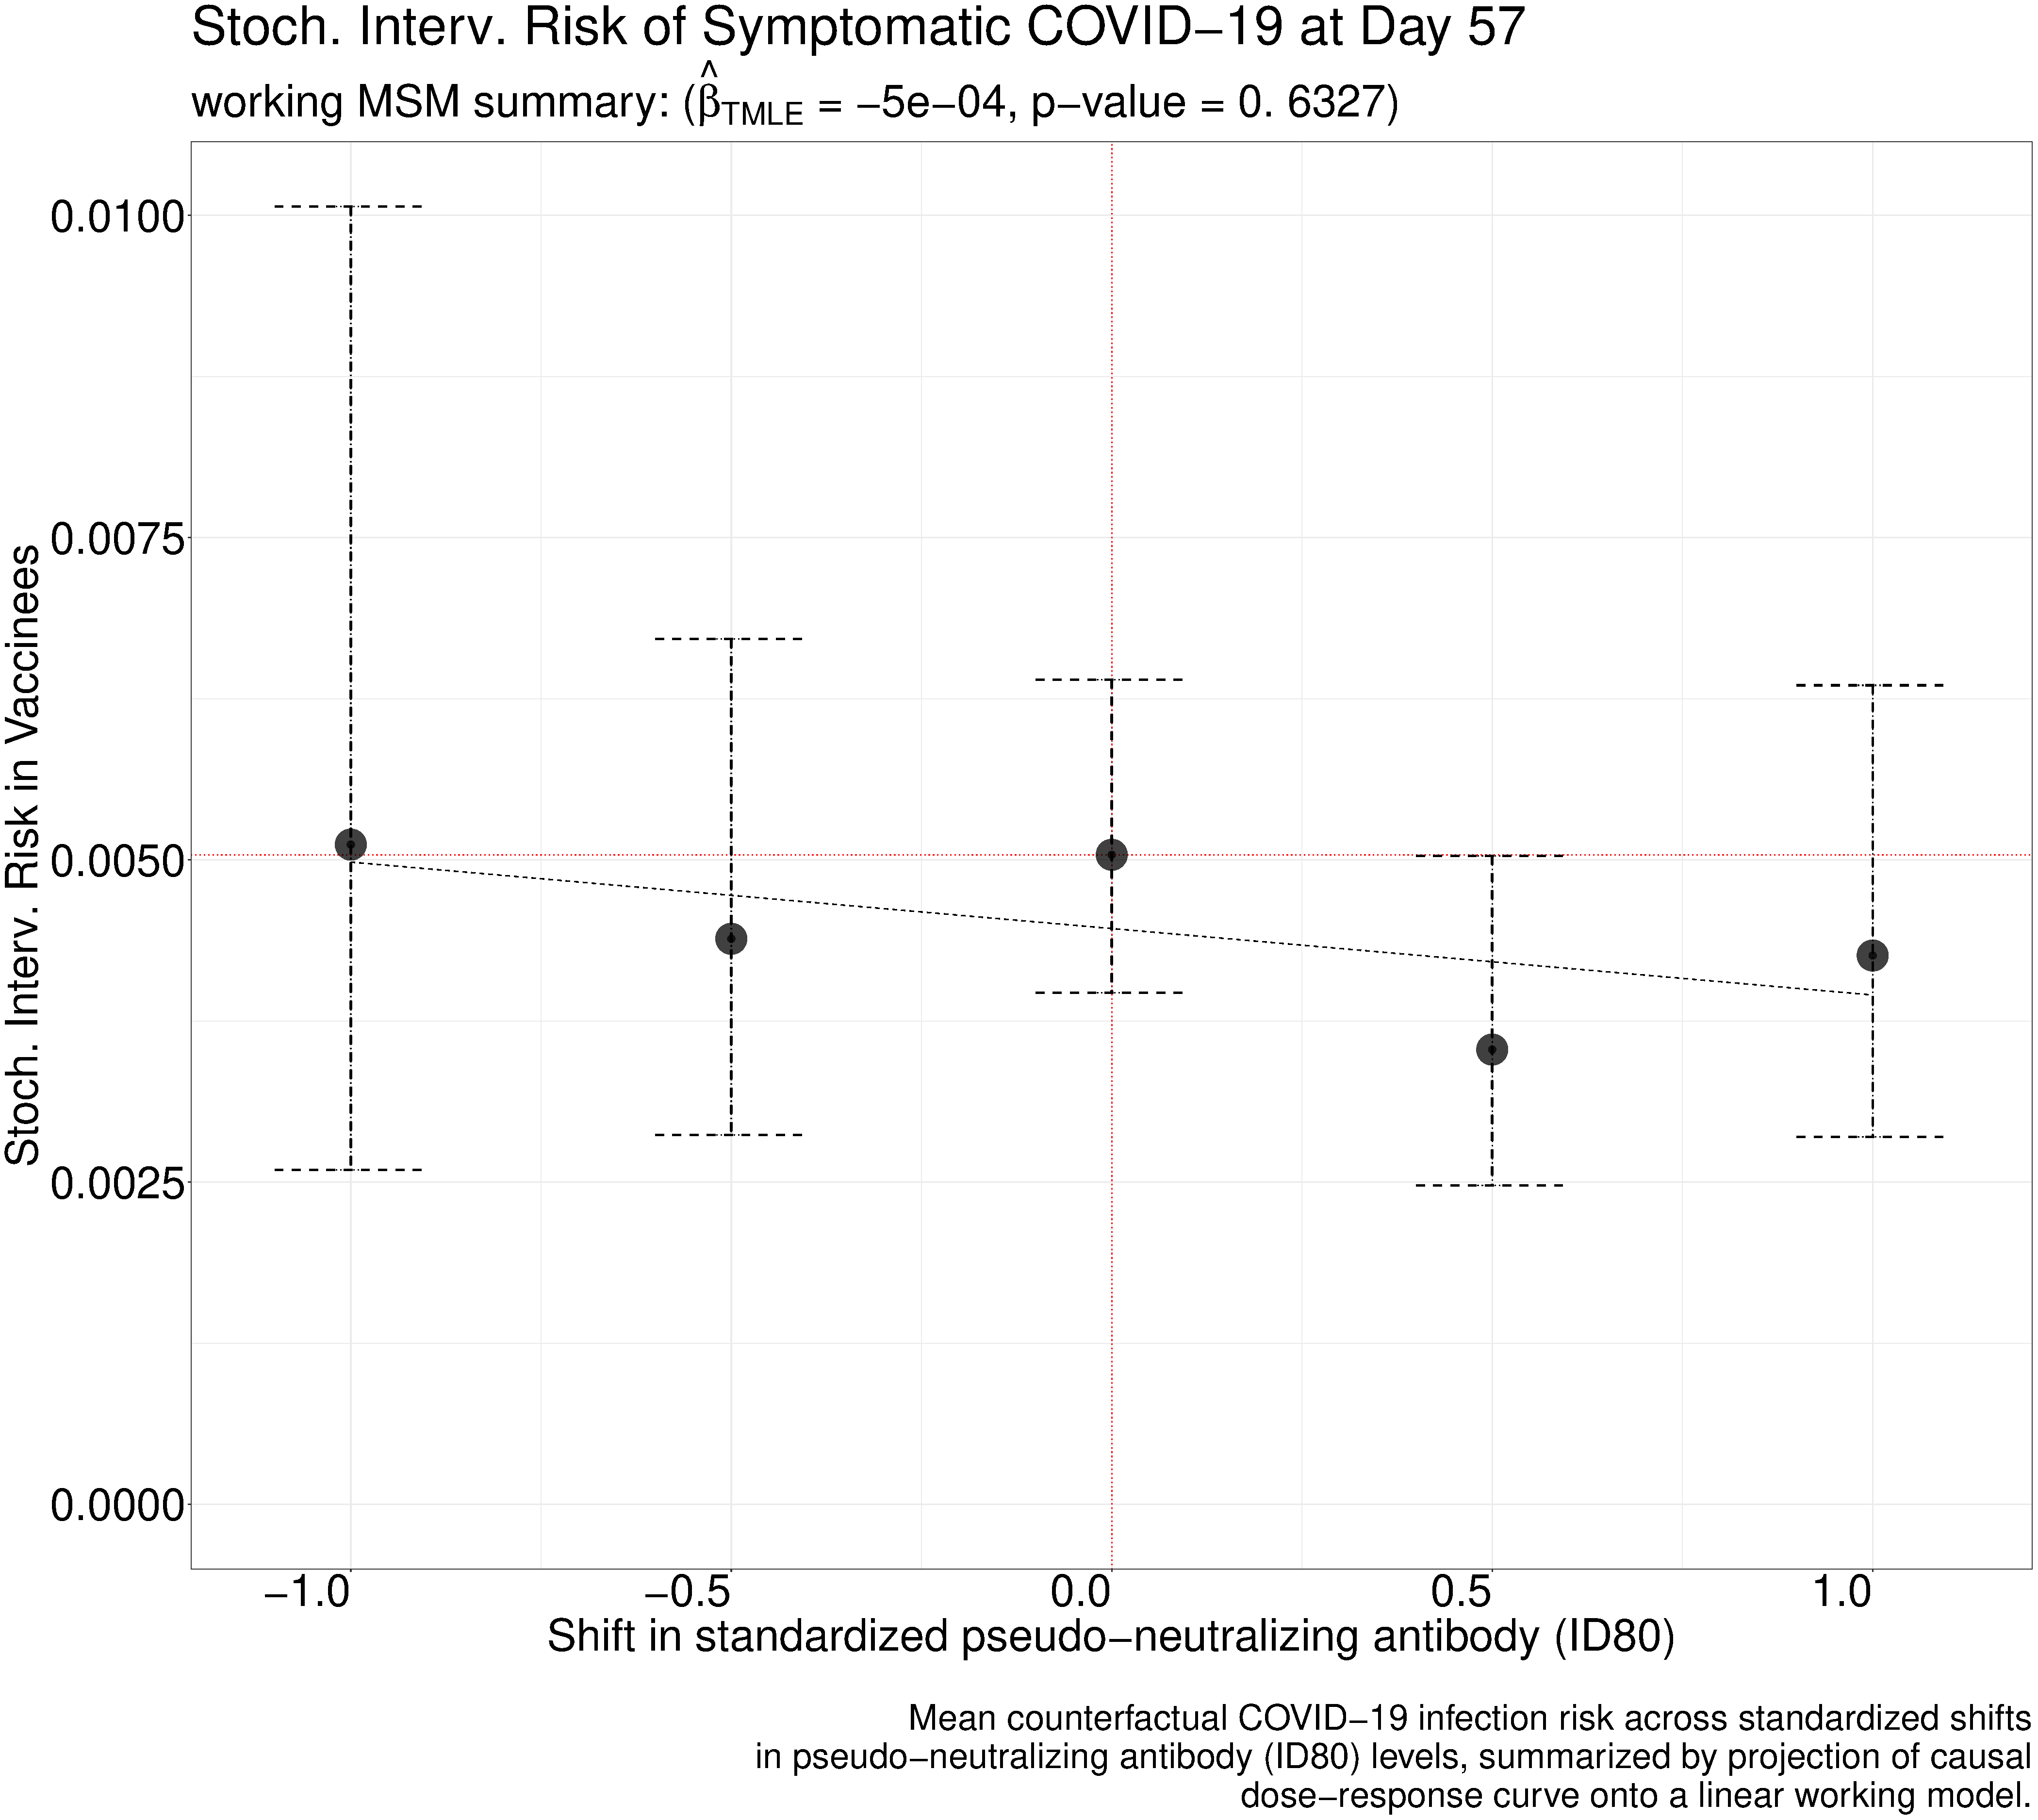
\includegraphics[width=0.95\linewidth,]{mcop_risk_Day57pseudoneutid80}
  \caption{Stochastic interventional risk estimates, with confidence intervals,
  for pseudo-neutralizing antibody (ID80) at Day 57}
  \label{fig:marker4-risk-day57}
\end{figure}

\begin{figure}[H]
  \centering
  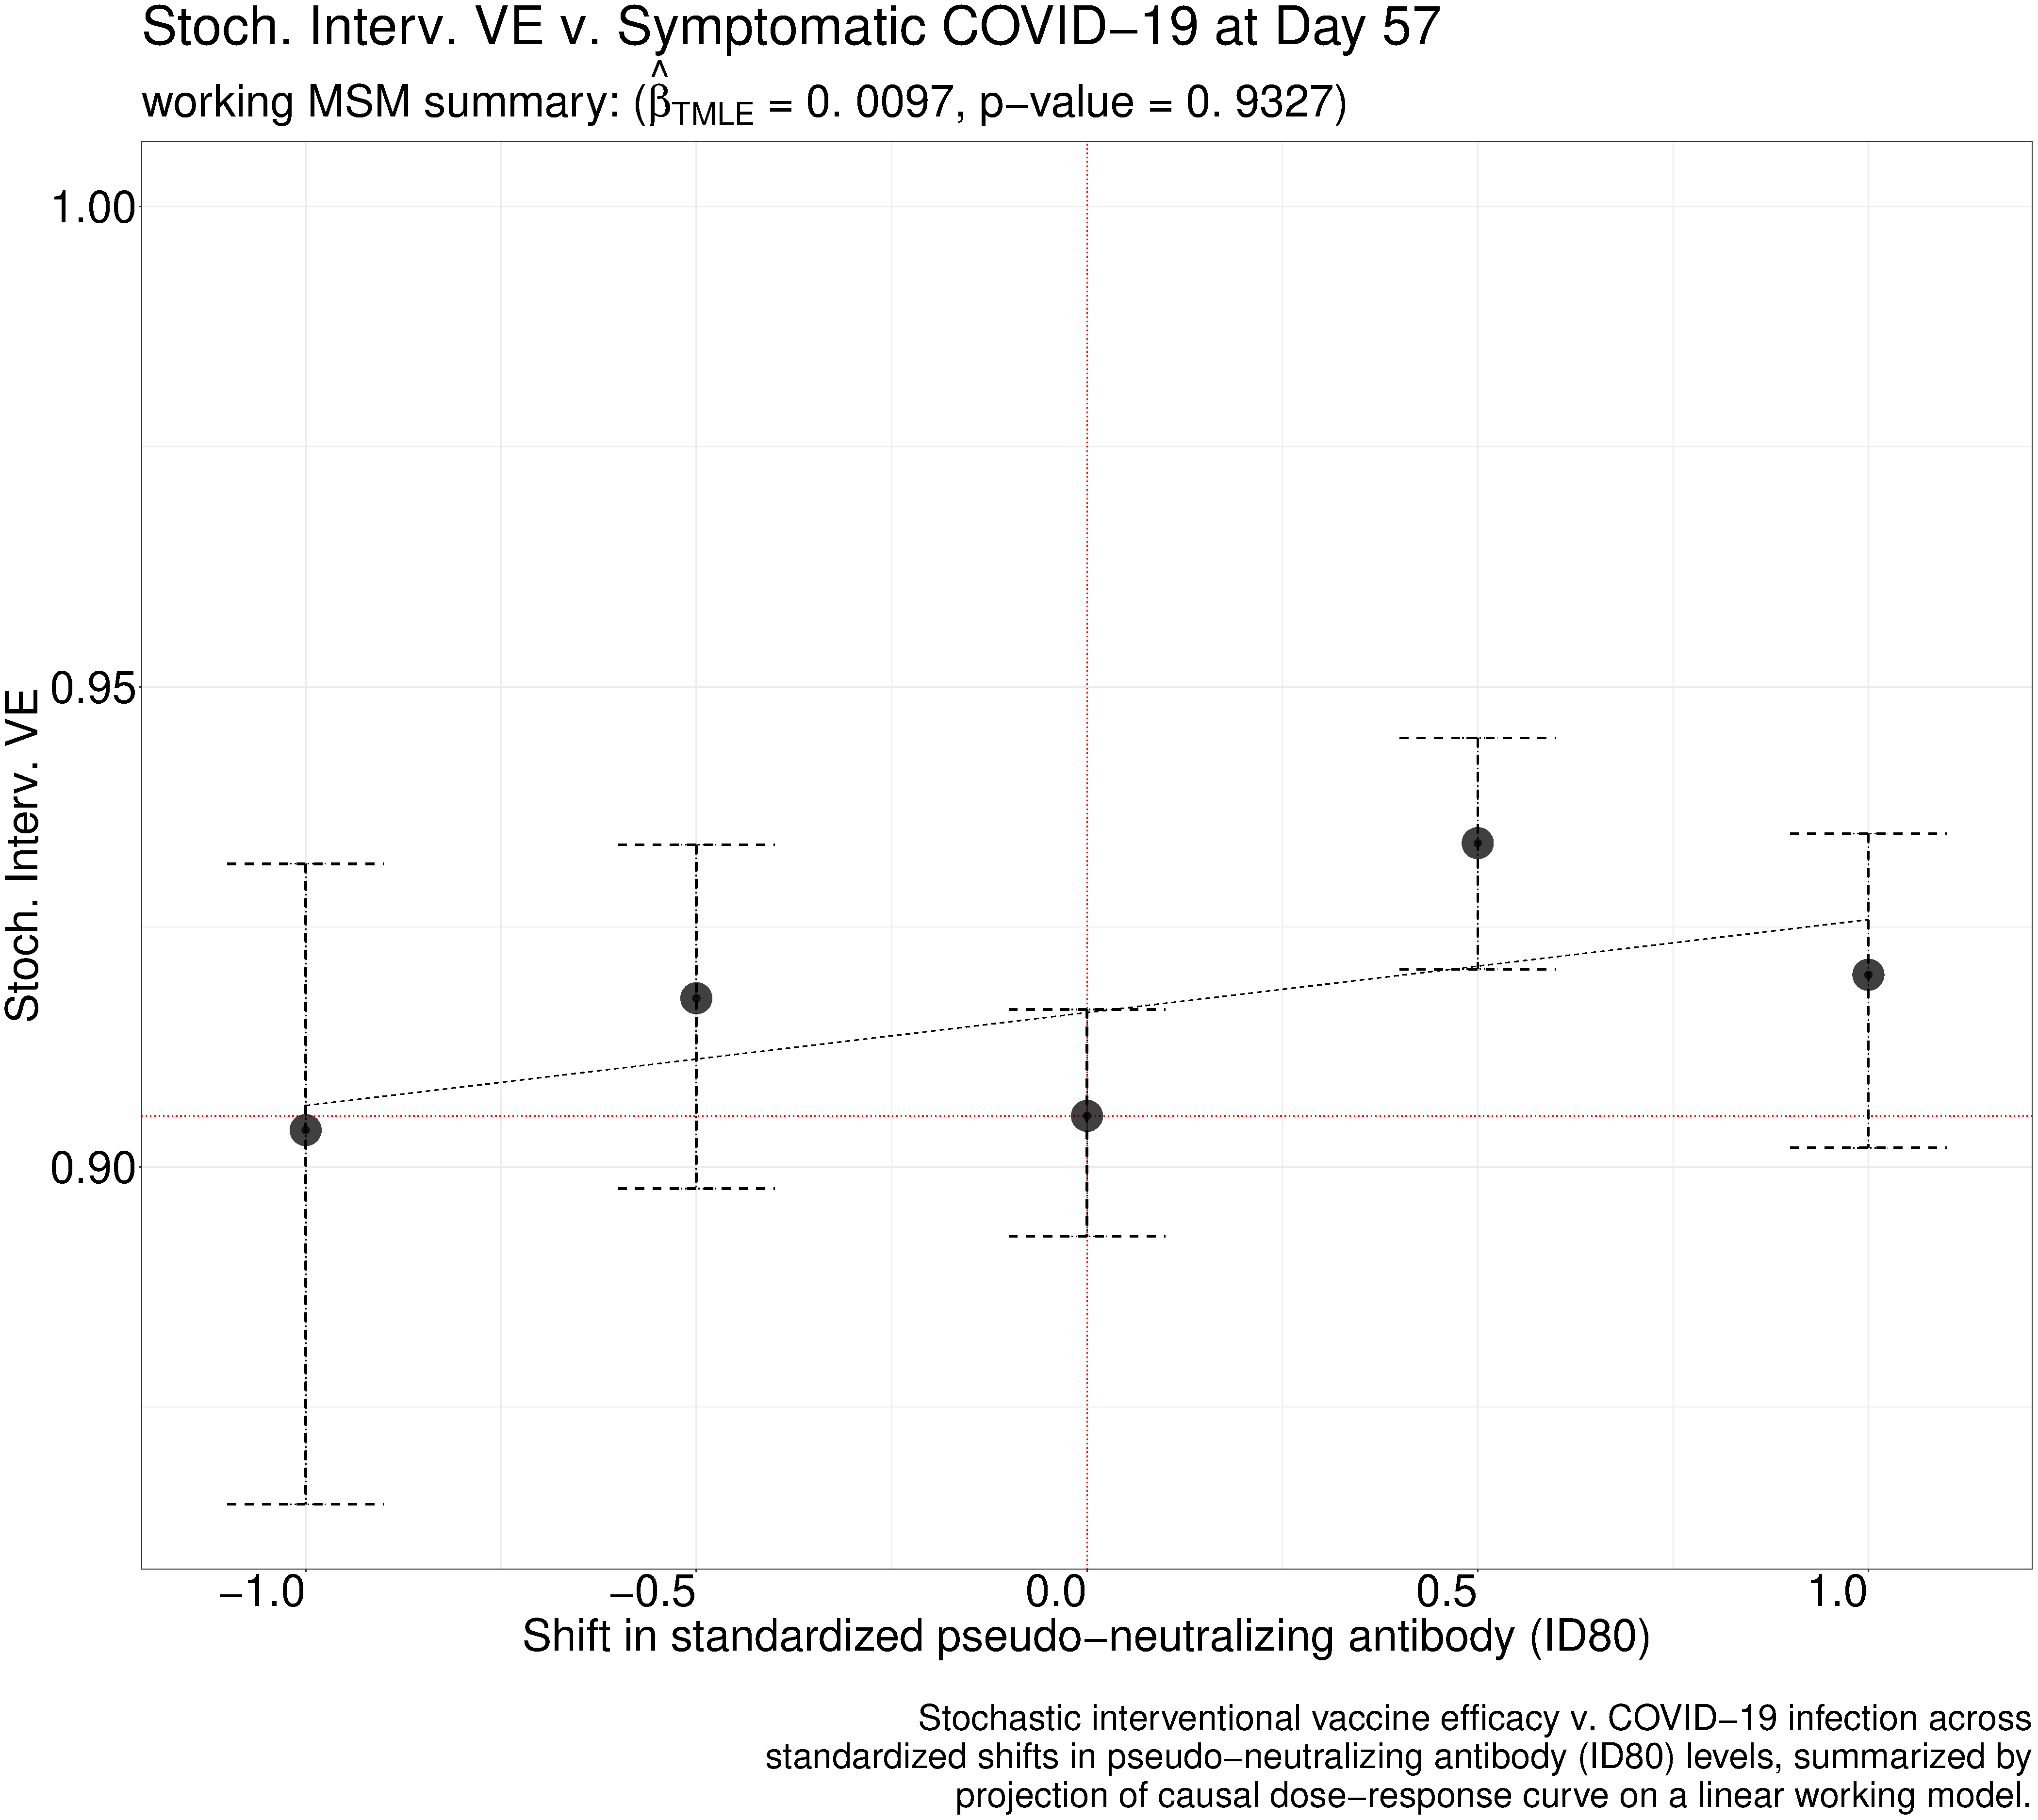
\includegraphics[width=0.95\linewidth,]{mcop_sve_Day57pseudoneutid80}
  \caption{Stochastic interventional VE estimates, with confidence intervals,
  for pseudo-neutralizing antibody (ID80) at Day 57}
  \label{fig:marker4-sve-day57}
\end{figure}
